\documentclass[11pt]{article}

% ---- CeAI style (provides geometry, boxes, tikz, etc.) ----
\usepackage{ceai}

% ---- Additional packages ----
\usepackage{listings}
\usepackage{fontawesome5}
\usepackage{booktabs}
\usepackage{tabularx}
\usepackage{multicol}
\usepackage{graphicx}
\usepackage[super]{nth}

% ---- Listings style for bash / terminal ----
\lstdefinestyle{term}{
  basicstyle=\ttfamily\small,
  backgroundcolor=\color{gray!8},
  frame=single,
  framerule=0.4pt,
  rulecolor=\color{gray!60},
  breaklines=true,
  columns=fullflexible,
  showstringspaces=false,
  commentstyle=\color{green!50!black},
  morecomment=[l]{\#},
  xleftmargin=4pt,
  xrightmargin=4pt,
  aboveskip=8pt,
  belowskip=4pt,
}

% ---- Shortcuts ----
\newcommand{\cmd}[1]{\texttt{\$ #1}}
\newcommand{\key}[1]{\keystroke{#1}}
\newcommand{\keystroke}[1]{%
  \tikz[baseline=(key.base)]{%
    \node[draw, rounded corners=2pt, inner sep=2pt, fill=gray!10,
          font=\ttfamily\small] (key) {#1};%
  }%
}

% ---- Title ----
\title{\textbf{Tutorial 05C: Concrete Strength --- Let's Do Prediction}\\[4pt]
       {\large AI Agentic Workflow for a First ML Baseline}}
\author{CE 488/5588 --- Applied Artificial Intelligence}
\date{Spring 2026}

\begin{document}
\maketitle

\begin{def-box}
\textbf{Overview - From exploration to prediction.}
In Tutorial 05B, you used OpenCode to discover that the concrete compressive-strength dataset is sparse, age-imbalanced, and physically time dependent.  In this tutorial, you will take the next step: use an AI coding agent to build a \textbf{first predictive pipeline}.  The goal is not to claim a deployable engineering model.  The goal is to learn the workflow: feature engineering, preprocessing, model training, testing, plotting, and critical interpretation.
\end{def-box}

\begin{ch-box}
By the end of this tutorial you will be able to:
\begin{enumerate}[nosep]
  \item Convert engineering insight into model features such as $\log(t)$ and a cement--water ratio.
  \item Use normalized, dimensionless inputs in a split-safe machine-learning pipeline.
  \item Train a small multilayer perceptron (MLP) regressor for concrete strength.
  \item Evaluate predictions using regression metrics and plots.
  \item Explain why sparse concrete data makes naive train/test accuracy easy to overinterpret.
\end{enumerate}
\end{ch-box}

% ===========================================================
\section{Why Prediction Comes After Exploration}
\label{sec:why-prediction}

Tutorial 05B ended with a warning: this dataset has a supervised learning structure, but the statistical situation is fragile.  There are 1,030 cleaned observations, 427 unique mixture designs, severe concentration at 28 days, and very few repeated measurements for the same mixture and age.  This means a model can produce attractive test metrics while still learning patterns that do not generalize reliably to new mixtures or unusual curing ages.

\begin{alert-box}
\textbf{Baseline mindset.}  In this tutorial, ``prediction'' means \emph{first baseline}, not final engineering authority.  We use a naive random 70/30 split because it is simple and familiar, but it can place related mixtures in both training and testing.  That makes the test set easier than a true new-mixture deployment problem.
\end{alert-box}

The important lesson is to build a pipeline that is honest about its assumptions.  We will deliberately use a cheap approach first, then discuss what research-oriented students could do next.

% ===========================================================
\section{Dataset Recap}
\label{sec:dataset-recap}

We continue using the UCI Concrete Compressive Strength dataset at:

\begin{lstlisting}[style=term]
Tutorials/UCI-Concrete Data/Concrete_Data_CSV.csv
\end{lstlisting}

The useful columns are the seven mixture components, curing age, and measured compressive strength.  Two derived columns, \texttt{f'c at 28 day} and \texttt{NSC}, are excluded from the baseline model because they are not raw mixture inputs and could create leakage or a different task.

\begin{center}
\begin{tabularx}{0.95\textwidth}{l X}
\toprule
\textbf{Role} & \textbf{Columns} \\
\midrule
Mixture inputs & Cement, slag, fly ash, water, superplasticizer, coarse aggregate, fine aggregate \\
Time input & Age (days), transformed to $\log(\text{age})$ \\
Engineered ratio & \texttt{cement\_to\_water} $= \text{cement}/\text{water}$ \\
Target & Concrete compressive strength (MPa) \\
Excluded & \texttt{f'c at 28 day}, \texttt{NSC} \\
\bottomrule
\end{tabularx}
\end{center}

% ===========================================================
\section{Feature Engineering: Cheap Physics-Aware Inputs}
\label{sec:features}

The MLP sees numbers, not civil-engineering context.  Feature engineering is how we inject a small amount of domain knowledge into a cheap baseline.

\begin{def-box}
\textbf{Age feature.}  Concrete strength grows quickly at early ages and more slowly later.  A simple way to reflect this diminishing rate is to replace raw age $t$ with
\[
  \log(t), \qquad t > 0.
\]
This does not force the model to be physically correct, but it gives the model a more useful representation of curing time.
\end{def-box}

\begin{def-box}
\textbf{Cement--water ratio.}  Water strongly affects concrete strength.  A simple engineered feature is
\[
  \texttt{cement\_to\_water} = \frac{\text{cement}}{\text{water}}.
\]
In a later research project, you might compare this with binder/water ratio, where binder includes cement, slag, and fly ash.
\end{def-box}

The remaining model inputs are normalized inside the machine-learning pipeline using \texttt{StandardScaler}.  Normalization makes the features dimensionless from the neural network's perspective, so cement measured near hundreds of kg/m$^3$ does not dominate a ratio or a log-age feature simply because of scale.

\begin{alert-box}
\textbf{Preprocessing guardrail.}  The scaler must be fit only on the training data.  Fitting it on the full dataset before splitting would leak information from the test set into the training process.  The companion code avoids this by using \texttt{Pipeline(StandardScaler(), MLPRegressor(...))}.
\end{alert-box}

% ===========================================================
\section{The Modular Prediction Workflow}
\label{sec:workflow}

The code for this tutorial is intentionally modular.  Students run one command, but the agent-created workflow separates data loading, feature engineering, model training, evaluation, and plotting.

\begin{center}
\begin{tabular}{l l}
\toprule
\textbf{File} & \textbf{Purpose} \\
\midrule
\texttt{Tutorials/concrete\_prediction/data.py} & Load and clean the CSV \\
\texttt{Tutorials/concrete\_prediction/features.py} & Create $\log(\text{age})$ and \texttt{cement\_to\_water} \\
\texttt{Tutorials/concrete\_prediction/model.py} & Split data and train the MLP pipeline \\
\texttt{Tutorials/concrete\_prediction/evaluate.py} & Compute R$^2$, MAE, and RMSE \\
\texttt{Tutorials/concrete\_prediction/plots.py} & Create regression diagnostic plots \\
\texttt{Tutorials/concrete-prediction/run\_prediction.py} & Student-facing command-line script \\
\bottomrule
\end{tabular}
\end{center}

\begin{ex-box}
\textbf{OpenCode prompt: inspect the workflow.}
\begin{lstlisting}[style=term]
Read the files in Tutorials/concrete_prediction and Tutorials/concrete-prediction/run_prediction.py.
Explain the data flow from CSV loading to feature engineering, train/test split, MLP training, metrics, and plot generation.
Pay special attention to where normalization is fit.
\end{lstlisting}
\end{ex-box}

% ===========================================================
\section{Run a Smoke Test}
\label{sec:smoke-test}

Before training the full baseline, run a quick smoke test.  A smoke test does not prove the model is good.  It proves the whole pipeline executes: load data, create features, split, train a small model, compute metrics, and write at least one plot.

\begin{lstlisting}[style=term]
python Tutorials/concrete-prediction/run_prediction.py --smoke-test
\end{lstlisting}

\begin{ex-box}
\textbf{OpenCode prompt: run the smoke test.}
\begin{lstlisting}[style=term]
Run the smoke-test command for Tutorial05C. Report:
- cleaned row count
- feature names
- excluded columns
- train/test split sizes
- train and test R^2, MAE, and RMSE
- generated plot filenames
If the command fails, diagnose and fix the root cause.
\end{lstlisting}
\end{ex-box}

% ===========================================================
\section{Train the Baseline MLP}
\label{sec:train-mlp}

The baseline model is a tabular regression MLP.  The data is randomly shuffled and split 70/30 into training and testing.  The model uses standardized features and a small neural network:

\begin{lstlisting}[style=term]
Pipeline([
    ("scaler", StandardScaler()),
    ("mlp", MLPRegressor(hidden_layer_sizes=(64, 32),
                         activation="relu",
                         solver="adam",
                         max_iter=1000,
                         early_stopping=True,
                         random_state=42))
])
\end{lstlisting}

Run the full baseline:

\begin{lstlisting}[style=term]
python Tutorials/concrete-prediction/run_prediction.py
\end{lstlisting}

The current reference run produced the following output on the course machine:

\lstinputlisting[style=term]{concrete-prediction-output.txt}

\begin{alert-box}
\textbf{Interpret metrics carefully.}  A test R$^2$ near 0.89 looks encouraging, but the random split is not a strict test of new-mixture generalization.  Because the dataset is sparse and related mixture designs may appear in both train and test, the metric is best read as evidence that the workflow runs and captures broad patterns, not proof of deployment-ready accuracy.
\end{alert-box}

\begin{ex-box}
\textbf{OpenCode prompt: train and summarize.}
\begin{lstlisting}[style=term]
Run python Tutorials/concrete-prediction/run_prediction.py.
Summarize the metrics as a regression problem. Explain what R^2, MAE, and RMSE mean in MPa units.
Then explain why this random 70/30 split may overstate generalization for sparse concrete mixtures.
\end{lstlisting}
\end{ex-box}

% ===========================================================
\section{Regression Evaluation Plots}
\label{sec:plots}

Because this is a regression task, the correct plots are regression diagnostics.  We do \emph{not} use ROC curves, confusion matrices, precision, recall, or classification accuracy unless we deliberately turn strength into categories.  That is not the baseline task here.

\begin{figure}[htbp]
\centering
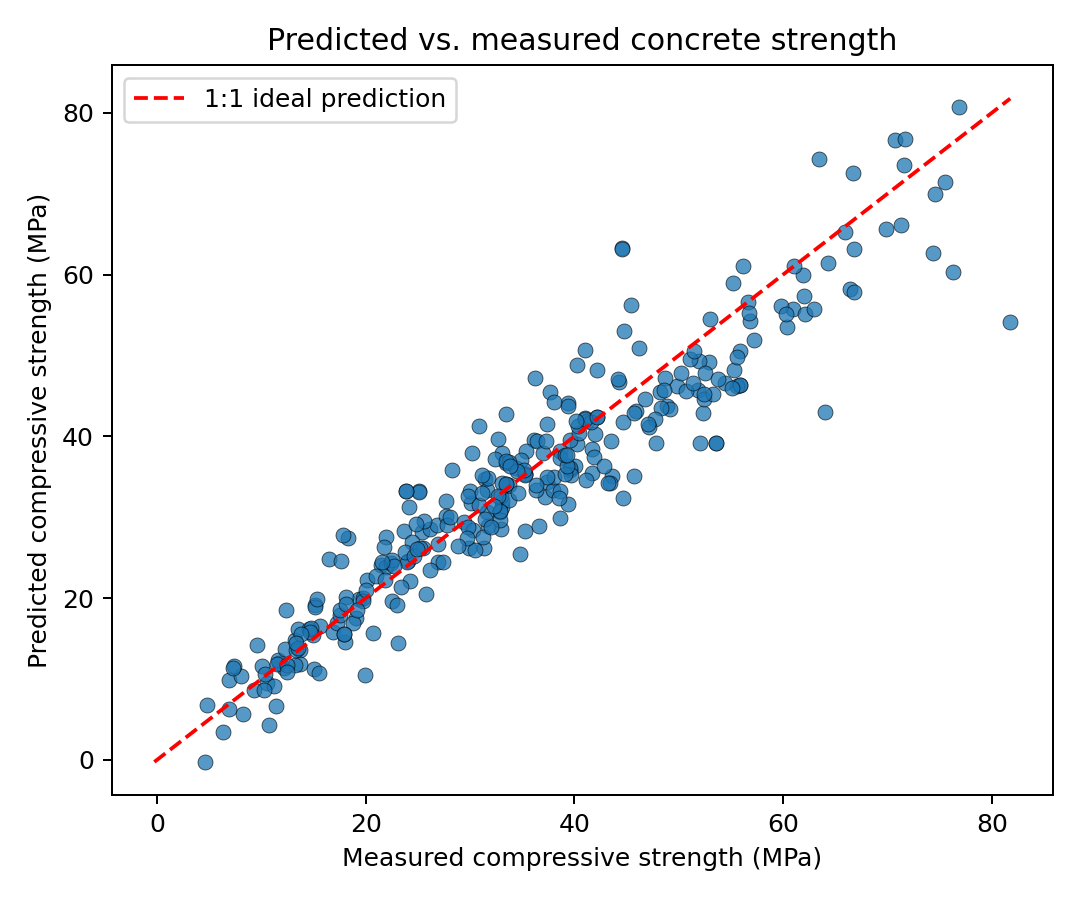
\includegraphics[width=0.78\textwidth]{concrete-prediction-assets/predicted_vs_actual.png}
\caption{Predicted versus measured compressive strength.  Points close to the dashed 1:1 line indicate better predictions; large vertical deviations indicate larger prediction errors.}
\label{fig:predicted-vs-actual}
\end{figure}

\begin{figure}[htbp]
\centering
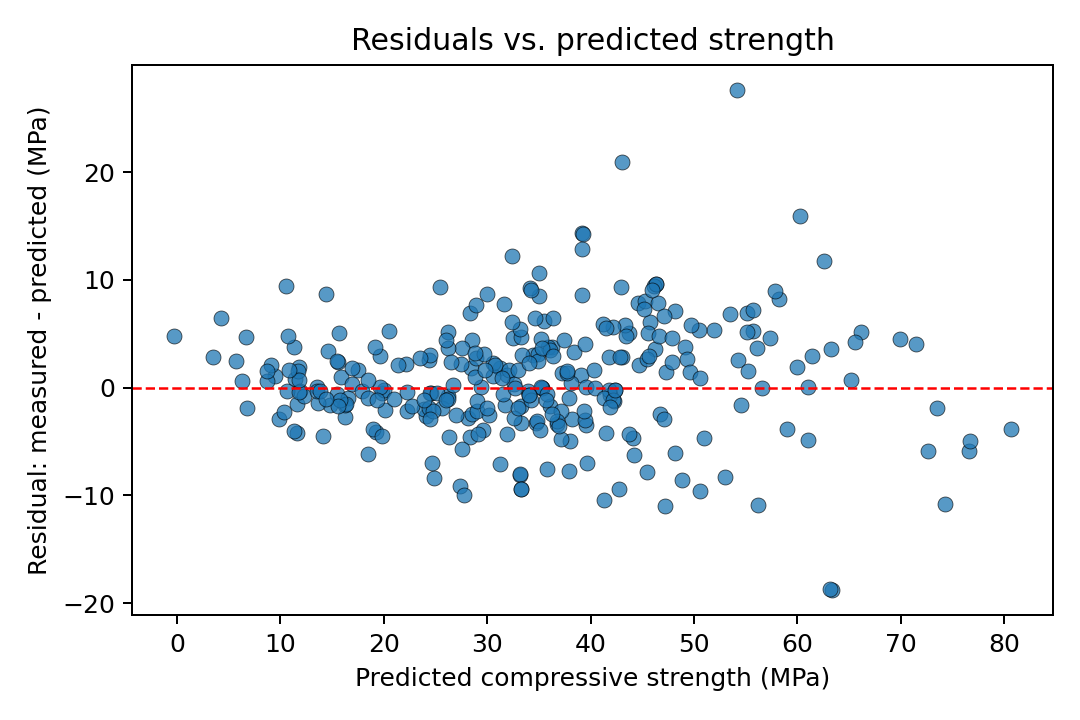
\includegraphics[width=0.78\textwidth]{concrete-prediction-assets/residuals_vs_predicted.png}
\caption{Residuals versus predicted strength.  This diagnostic checks whether errors are centered around zero or show systematic patterns across predicted strength.}
\label{fig:residuals-vs-predicted}
\end{figure}

\begin{figure}[htbp]
\centering
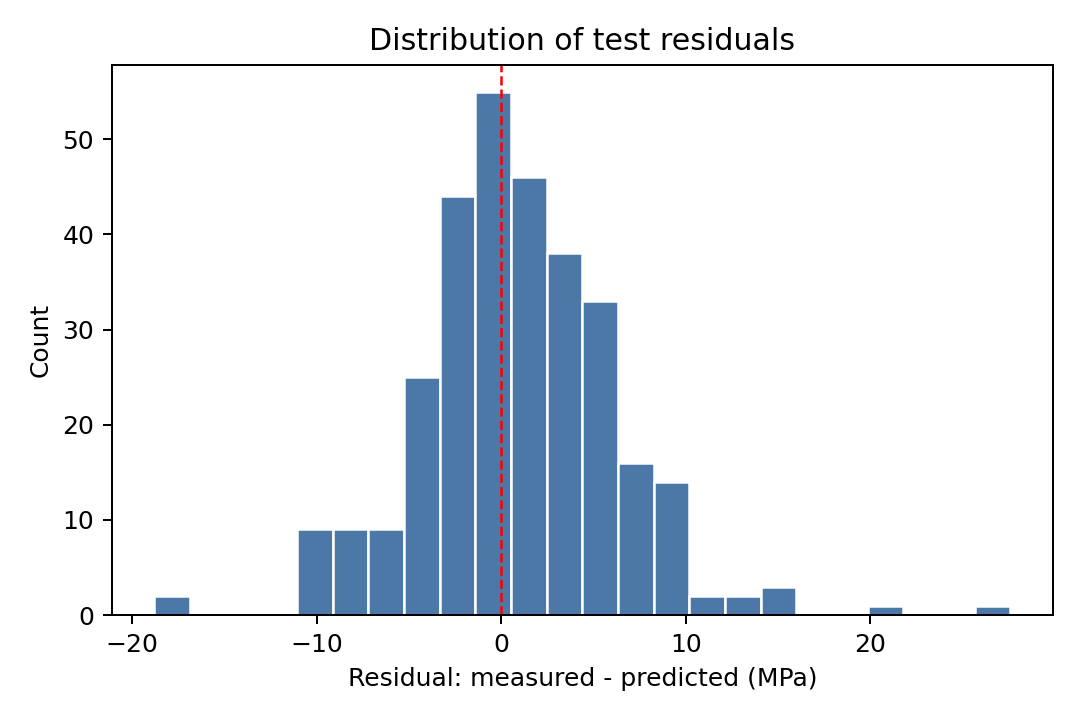
\includegraphics[width=0.78\textwidth]{concrete-prediction-assets/residual_histogram.png}
\caption{Histogram of residuals on the test set.  A narrow distribution centered near zero indicates smaller unbiased errors, while skew or heavy tails suggest systematic misses.}
\label{fig:residual-histogram}
\end{figure}

\begin{figure}[htbp]
\centering
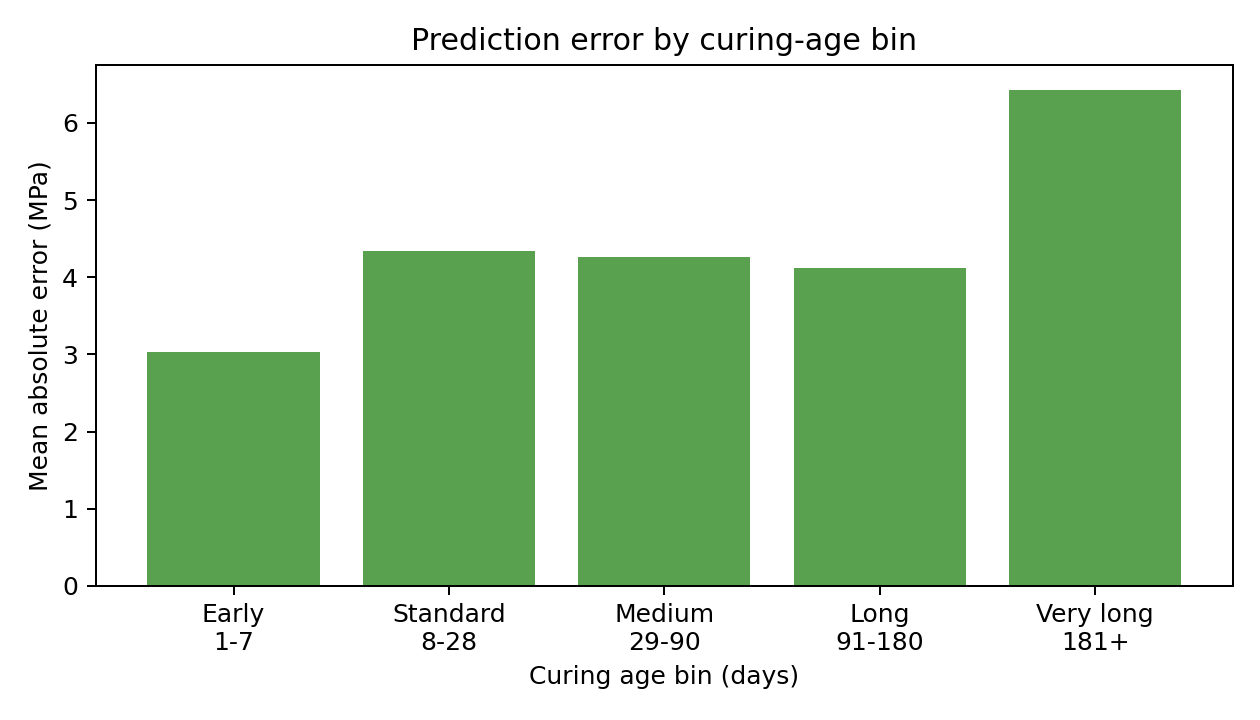
\includegraphics[width=0.78\textwidth]{concrete-prediction-assets/error_by_age_bin.png}
\caption{Mean absolute prediction error by curing-age bin.  This view matters because the dataset is age-imbalanced, with many 28-day samples and few long-term samples.}
\label{fig:error-by-age-bin}
\end{figure}

\begin{figure}[htbp]
\centering
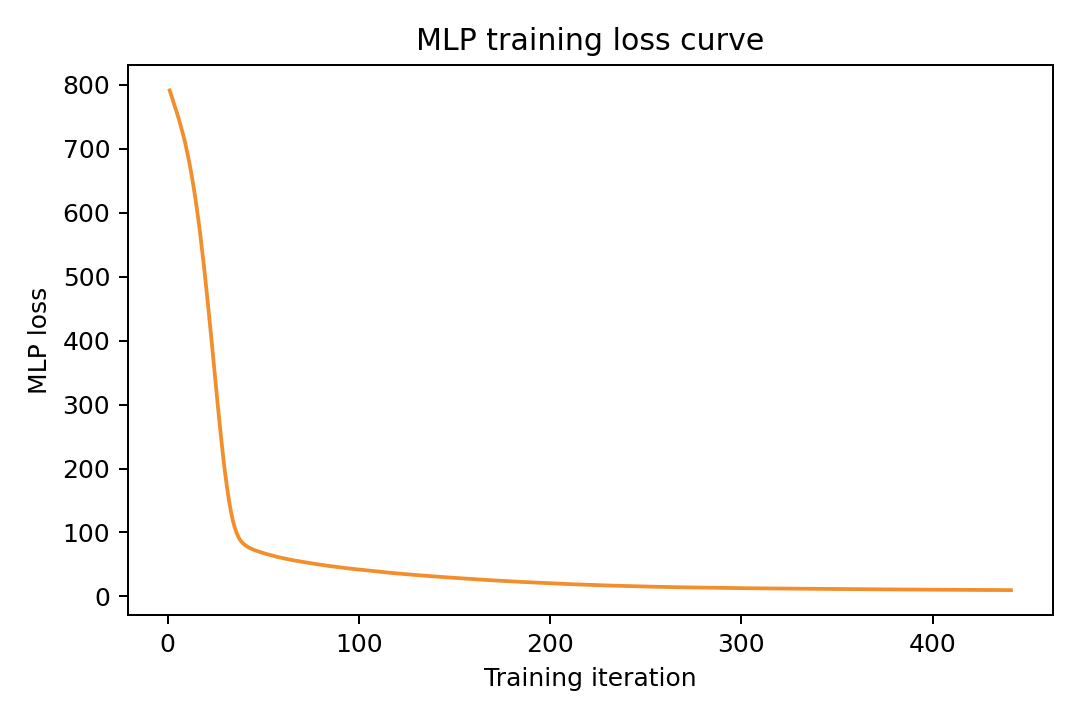
\includegraphics[width=0.78\textwidth]{concrete-prediction-assets/training_loss_curve.png}
\caption{MLP training loss curve.  The curve summarizes optimization progress, but it does not by itself prove that the model generalizes physically.}
\label{fig:training-loss}
\end{figure}

\begin{ex-box}
\textbf{OpenCode prompt: critique the plots.}
\begin{lstlisting}[style=term]
Inspect the plots in Tutorials/concrete-prediction-assets.
For each plot, explain what it tells us about model performance.
Then identify at least two ways the plots could hide problems caused by sparse data or age imbalance.
\end{lstlisting}
\end{ex-box}

% ===========================================================
\section{What This Baseline Teaches}
\label{sec:what-learned}

This baseline is intentionally simple, but it contains the core pieces of a real ML workflow.

\begin{enumerate}[nosep]
  \item \textbf{Feature engineering matters.}  The variables $\log(\text{age})$ and \texttt{cement\_to\_water} encode simple engineering intuition before the model sees the data.
  \item \textbf{Preprocessing is part of the model.}  Normalization must be fit on training data only, so it belongs inside the pipeline.
  \item \textbf{Regression metrics have units and context.}  MAE and RMSE are measured in MPa, while R$^2$ is unitless.
  \item \textbf{A naive random split is convenient but weak.}  It is useful for a quick tutorial but not the final word for sparse mixture data.
\end{enumerate}

\begin{alert-box}
\textbf{No ROC for this baseline.}  ROC curves evaluate classifiers.  Concrete compressive strength is predicted here as a continuous MPa value.  If a future tutorial defines classes such as low-, normal-, and high-strength concrete, then classification metrics could be introduced explicitly.  They are not appropriate for this baseline regression workflow.
\end{alert-box}

% ===========================================================
\section{Thinking Beyond the Naive Split}
\label{sec:beyond-naive}

The central challenge from Tutorial 05B remains: sparsity.  Random shuffling is a naive but accessible way to start.  Once the workflow is running, students should ask harder questions.

\begin{def-box}
\textbf{Alternative evaluation.}  A stricter evaluation would split by mixture design, so the same mixture does not appear in both training and testing.  This asks a harder question: can the model predict strength for a truly new mixture?
\end{def-box}

\begin{def-box}
\textbf{Data augmentation.}  Sparse longitudinal data may benefit from physics-aware augmentation, interpolation along plausible curing curves, or synthetic mixtures constrained by domain knowledge.  Augmentation must be designed carefully; otherwise it can simply manufacture false confidence.
\end{def-box}

\begin{def-box}
\textbf{Support vector machines.}  For small tabular datasets, support vector regression can be a strong classical alternative to neural networks.  A future comparison could train both \texttt{MLPRegressor} and \texttt{SVR} under the same preprocessing and split.
\end{def-box}

% ===========================================================
\section{Research-Oriented Extensions}
\label{sec:research-extensions}

For research-oriented students, the most interesting direction is to stop treating time as merely another tabular feature.  Concrete strength development is a curve.

One possible backbone is
\[
  f_c(t) = f_{c28}\,\frac{t}{a + b t},
\]
where $f_c(t)$ is compressive strength at age $t$, $f_{c28}$ is a 28-day reference strength, and $a$ and $b$ control the time-dependent curve shape.  Instead of fitting a separate curve for each sparse mixture, a physics-informed model could learn
\[
  a = g_a(\text{mixture}), \qquad b = g_b(\text{mixture}),
\]
where $g_a$ and $g_b$ are nonlinear functions of cement, water, slag, fly ash, aggregates, and admixtures.

There is one important detail: the simple expression above does not automatically satisfy $f_c(28)=f_{c28}$ unless $a+28b=28$.  A calibrated research model would either enforce that constraint or use a 28-day-normalized form such as
\[
  f_c(t) = f_{c28}\,
  \frac{t/(a+b t)}{28/(a+28b)}.
\]
This is exactly why the backbone belongs in a research extension rather than in today's quick baseline.

\begin{alert-box}
\textbf{Physics-informed does not mean automatically correct.}  A physics-informed backbone can improve extrapolation only if it is calibrated, validated, and checked against the data-generating assumptions.  It is a research model, not a shortcut around validation.
\end{alert-box}

Another possible future direction is a memory model such as a long short-term memory network.  However, this dataset is not a clean sequence dataset in the usual sense.  Most mixtures have only one to three ages.  An LSTM would be speculative unless the data are reorganized into meaningful curing histories or augmented with additional sequential observations.

\begin{ex-box}
\textbf{OpenCode prompt: propose future models.}
\begin{lstlisting}[style=term]
Based on Tutorial05B sparsity findings and Tutorial05C baseline results, propose three future modeling directions:
1. a stricter train/test split,
2. a classical small-data model such as SVR,
3. a physics-informed time-dependent model using f_c(t)=f_c28*t/(a+b*t), including the 28-day normalization issue.
For each direction, state the benefit, risk, and validation requirement.
\end{lstlisting}
\end{ex-box}

% ===========================================================
\section{Reflection Questions}
\label{sec:reflection}

\begin{enumerate}
  \item Why is $\log(\text{age})$ a more physically motivated feature than raw age for concrete curing?
  \item Why must \texttt{StandardScaler} be fit only on the training split?
  \item What does MAE mean in MPa, and why might RMSE be larger?
  \item Why can a random 70/30 split be misleading for sparse mixture data?
  \item What evidence would convince you that a model generalizes to new mixture designs?
\end{enumerate}

% ===========================================================
\section{Looking Ahead}
\label{sec:looking-ahead}

You have now moved from data exploration to a working prediction baseline.  The workflow is useful because it is modular and testable: each stage can be inspected, run, and improved.  The next step is not simply to make the neural network bigger.  The next step is to design evaluation and model structure that respect the physics and sparsity of the problem.

\begin{def-box}
\textbf{Takeaway.}  A good AI-agentic workflow does not stop when the code runs.  It asks whether the code answers the right engineering question, whether the validation is honest, and whether the model structure matches the physical system.
\end{def-box}

% ===========================================================
% References
% ===========================================================

\begin{thebibliography}{9}

\bibitem{yeh1998}
I-Cheng Yeh, ``Modeling of strength of high performance concrete using artificial neural networks,'' \emph{Cement and Concrete Research}, Vol.~28, No.~12, pp.~1797--1808 (1998).

\bibitem{pedregosa2011}
F. Pedregosa et al., ``Scikit-learn: Machine Learning in Python,'' \emph{Journal of Machine Learning Research}, Vol.~12, pp.~2825--2830 (2011).

\bibitem{opencode2025}
opencode-ai, ``OpenCode: A powerful AI coding agent. Built for the terminal,'' \emph{GitHub}, 2025. Available: \url{https://github.com/opencode-ai/opencode}

\end{thebibliography}

\end{document}
